% !TEX encoding = UTF-8 Unicode
% !TEX root = project.tex

\section{Software Implementation}
\label{sec:setup}
\\
In this section, we would like to explain the implementation of Noodlr including the frontend and backend of the tool. Since Noodlr is a web based tool, we have divided this section into two namely:
\begin{enumerate}
    \item Noodlr frontend implementation
    \item Noodlr backend implementation
\end{enumerate}

Frontend can be accessed from anywhere with the help of a web browser that has Javascript enabled. For evaluation purposes, we used a laptop with Intel Core i7-2720QM CPU running at 2.2 GHz with 8 GB RAM, with Windows 7 professional operating system.\\

For the backend, implementation was done on a single laptop having an Intel Core i5 CPU running at 1.6 GHz with 4 GB RAM, with OSX El Capitan operating system.

\subsection{Frontend Implementation}
Noodlr was envisioned to be an interactive web based tool, so we decided to make use of JavaScript language to implement the front end of Noodlr. Since the objective of Noodlr was to provide an interactive interface which can be used by managers and developers, the interface was developed in D3.js\cite{d3js}. D3.js (D3 = Data-Driven Documents) is a JavaScript library for producing dynamic, interactive data visualizations in web browsers. It makes use of the widely implemented SVG, HTML5, and CSS standards. D3 provides hundreds of data visualization options, but our motive was to incorporate a style which can display the graph of packages, classes and methods showing the parent-child relationship (to show Package-Class and Class-method) as well as showing links with source and targets arrows (to show call dependencies). \\

A popular D3 style called Sankey style\footnote{\url{http://bl.ocks.org/wvengen/cab9b01816490edb7083}} was a good choice as per our requirement, as we wanted to have an expand-and-collapse functionality for our graph nodes. For example, if user double clicks on a class node, it should expand and draw all the method nodes and if he/she again double clicks on the top left corner on the particular class node, all its method nodes should collapse into one class node. We had to make changes in the Sankey D3 library to create this expand and collapse functionality.\\

In our design, every component(class, method and package) has a node with a different colour on the graph. All the package nodes contains class nodes embedded and all the class nodes contain the method nodes embedded. If user double clicks on the package (with green colour node), an animation will be shown with the package moving to the top left corner of the browser window and all the contained classes will pop out on the graph with orange colour nodes. If user double clicks on the class (with orange colour node), an animation will be shown with the class node moving to the top left corner and it will pop out all the methods on the graph (with violet colour nodes). Similarly, top left corner nodes which were created by the earlier actions can be double clicked to collapse related nodes on the graph.\\

Our custom Sankey style takes two JSON files as input. One file is the parent-child relationship file, with each node defined with various attributes in key-value pair form. For example, a class Class1 is defined as follows:

\begin{table}[h]
    \centering
    \begin{tabular}{lll}
        \{\\
        ``type'' & : & ``Class'',\\
        ``id'' & : & ``c1'',\\
        ``parent'' & : & ``p1'',\\
        ``name'' & : & ``Class\_1'',\\
        ``full\_name'' & :& ``p1.Class\_1''\\ 
        \}
    \end{tabular}
    \caption{\textbf{JSON node type 1}}
    \label{tab:node1}
\end{table}
  
 JSON node as shown in Table~\ref{tab:node1} states that this node is of type class, with id `c1' whose parent is package `p1' and name of this node is `Class\_1'. In this way, all packages, classes and methods are defined in a JSON file. Second file contains the links with source and target nodes defined in another JSON format. Format shown in Table~\ref{tab:node2} is of that JSON file.

\begin{table}[h!]
    \centering
    \begin{tabular}{lll}
        \{\\
        ``source'' & : & ``m1'',\\
        ``target'' & : & ``m2'',\\
        ``value'' & : & ``calls / depends on'',\\
        \}
    \end{tabular}
    \caption{\textbf{JSON node type 2}}
    \label{tab:node2}
\end{table}

In the JSON node shown in Table~\ref{tab:node2}, the source id and the target id are defined, with the kind of relationship they share as the value. For example, in the JSON node shown in Table~\ref{tab:node2}, method `m1' calls method `m2' and hence making a link on the graph. After these two input files are available, Noodlr calls custom Sankey style D3 library and renders the D3 graph on the user's screen.\\\\
From the Noodlr following properties can easily be observed:


\begin{table}[h]
\centering
\begin{tabular}{ll}
\hline
Property & Description\\
\hline
Shape & State of the node (Expanded/Collapsed)\\
Color & Type of node (Package, Class \& Method)\\
Height & Amount of linkages\\
Arrows & Caller to called node\\
Hovered text & Node description\\
\hline
\end{tabular}
\caption{Different measures \& their description in Noodlr.}
\label{tab:prop1}
\end{table}\\

To explain the properties shown in Table~\ref{tab:prop1}, we would like to use Figure \ref{fig:noodlr_ui}. As can be seen in Figure~\ref{fig:noodlr_ui}, Class\_1 is connected with Class\_2 and Class\_3 where Class\_1 method is calling some method of Class\_2 and a method of Class\_1 is calling a Class\_3 method. 

\begin{figure}[h!]
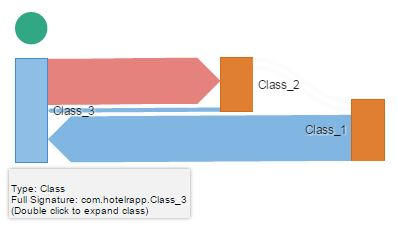
\includegraphics[width=8cm]{measures}
\caption{Noodlr User Interface}
\label{fig:noodlr_ui}
\end{figure}

\begin{enumerate}
    \item \textbf{Shape}: All the expanded nodes can be seen in the top left corner in circular shape. All the collapsed nodes are shown in a rectangular shape. In Figure~\ref{fig:noodlr_ui}, green coloured circle represents a package that contains Class\_1, Class\_2 and Class\_3.
    \item \textbf{Color}: Green represents `Package', Orange represents `Class', Violet represents `Method' and Light blue color represents hovered node.
    From arrows perspective, Red colored arrow represents current hovered node that is calling the other node at the target end of the arrow. Whereas the Light blue arrow represents current node being called by other node which is at the source end of the arrow.
    \item \textbf{Height}: Height of each rectangular node represents the number of links with respect to other nodes in the graph. Larger height of node means more links with other nodes in the graph.
    \item \textbf{Arrows}: Arrows play a vital role in Noodlr. Arrows represent which Node is calling/depends on which other node. Arrow's source is the caller node and target is the called node.
    \item \textbf{Hovered text}: Hovered text is used extensively in Noodlr and is used on each component. If any node is hovered, the hovered text shows some main characteristics like type, full signature and the action to be taken. On arrows, hovered text explains which node is calling which other node.
\end{enumerate}


Figure~\ref{fig:noodlr_ui_package} shows how the open call hierarchy graph visualization will look like for a small project when the nodes are all collapsed. We have selected a small project to make it easier to demonstrate in the limited space of the paper. In this view, it shows all the Java packages of the project. Since this is a small sample project, there are classes in the the project which are not in any Java packages, i.e., in the default package. That is shown as ``DEFAULT'' package in the figure. When all the packages represented by the green nodes are double-clicked, the image shown in Figure~\ref{fig:noodlr_ui_class} will show up. That is a partially expanded view where it shows the relationships between the Java classes in the project. This view can be further expanded to show up the methods present in the classes and their relationships. This view is shown in Figure~\ref{fig:noodlr_ui_method}. This is the completely expanded view of the graph and the highest granularity possible with the tool. A user can choose to expand only those packages of his interest and to see how relationships emerge from there. In all these 3 representations, the user can hover on any node to see all the nodes that it connects to and the detailed description of the node.


\begin{figure}[h!]
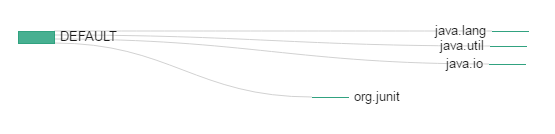
\includegraphics[width=8cm]{ui-package-view}
\caption{Noodlr UI: Package view (Fully collapsed)}
\label{fig:noodlr_ui_package}
\end{figure}

\begin{figure}[h!]
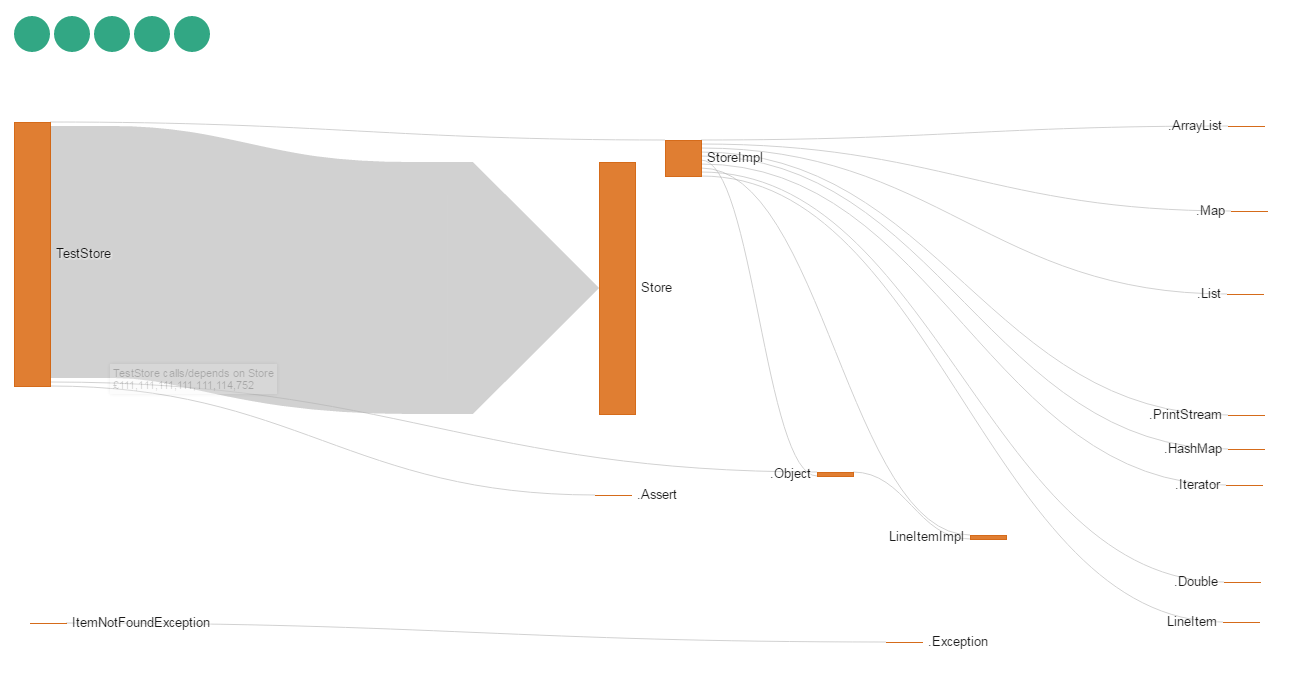
\includegraphics[width=8cm]{ui-class-view}
\caption{Noodlr UI: Class view (Partially expanded)}
\label{fig:noodlr_ui_class}
\end{figure}

\begin{figure}[h!]
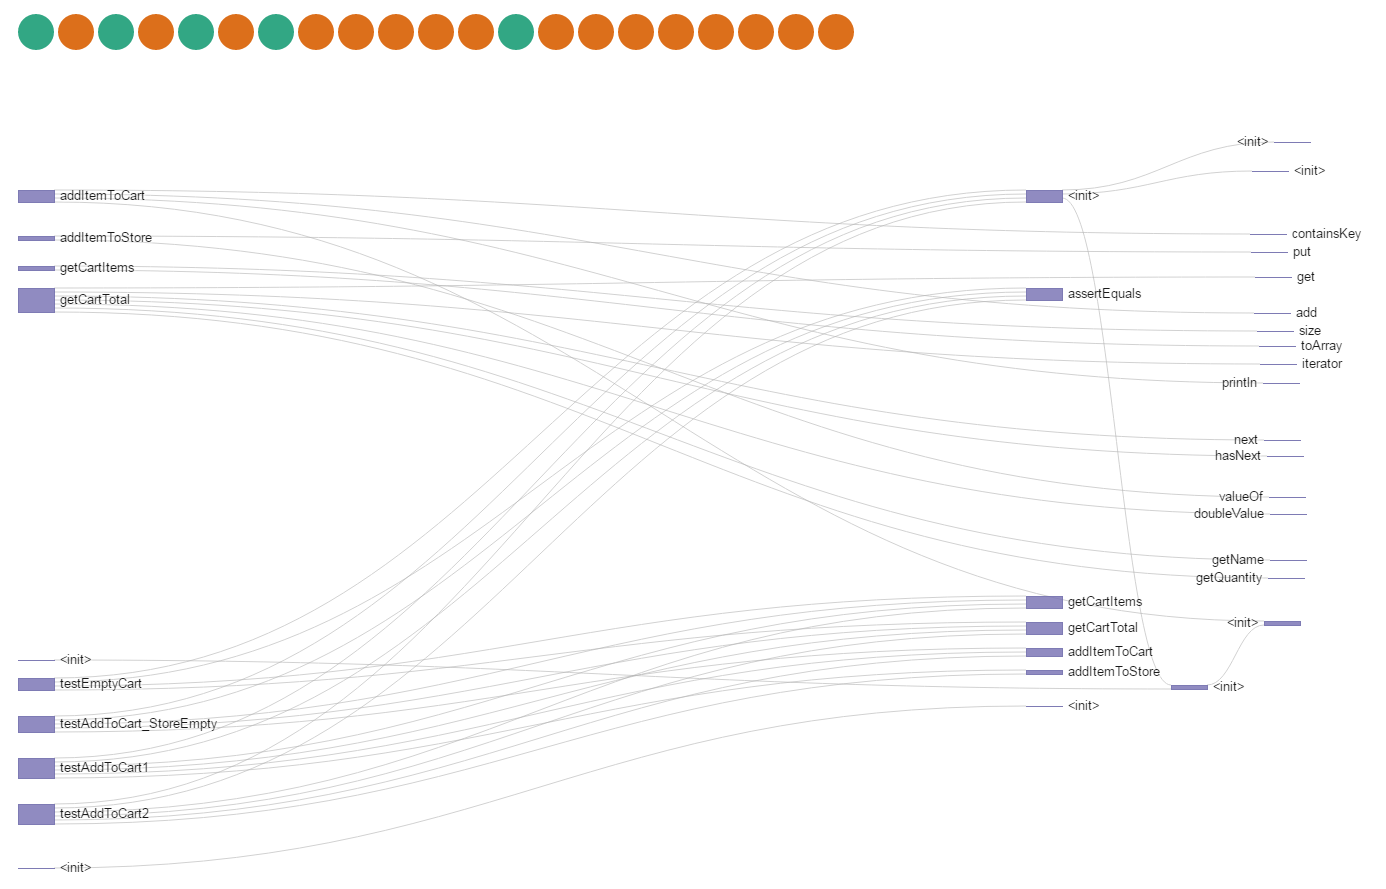
\includegraphics[width=8cm]{ui-method-view}
\caption{Noodlr UI: Method view (Fully expanded)}
\label{fig:noodlr_ui_method}
\end{figure}

\subsection{Backend implementation}

The backend implementation was done in Java and contains the logic to read the project files and create the graph of packages, classes and methods. Once the graph is generated, various graph algorithms such as the Kosaraju-Sharir algorithm and the Bron-Kerbosch algorithm were applied. This was to generate parts of the graph which is more defect-prone than others.\\

The first part of the process was to read an input jar file. Although there were multiple options to read files from a project, taking jar file as input seemed to be a straightforward choice for us given that the jar files are generated after the project is cleanly build without errors. Once the jar file is read, it is searched for class files and all class files are read using Apache Commons Byte Code Engineering Library (Apache Commons BCEL\texttrademark). All the methods are also read and their dependencies found along with the class to class dependencies. Using all the class to class dependencies and the method to method dependencies found using BCEL, a graph is constructed with vertexes as the classes or methods and edges as the relationship between them. \\

Once the graph was constructed, we implemented the required algorithms in Java to work on the graph to produce required results. The output produced by the Java implementation of the algorithms were fed to the frontend to produce the D3 graphs which could be displayed to the user.
